\documentclass{article}\usepackage[]{graphicx}\usepackage[]{color}
%% maxwidth is the original width if it is less than linewidth
%% otherwise use linewidth (to make sure the graphics do not exceed the margin)
\makeatletter
\def\maxwidth{ %
  \ifdim\Gin@nat@width>\linewidth
    \linewidth
  \else
    \Gin@nat@width
  \fi
}
\makeatother

\definecolor{fgcolor}{rgb}{0.345, 0.345, 0.345}
\newcommand{\hlnum}[1]{\textcolor[rgb]{0.686,0.059,0.569}{#1}}%
\newcommand{\hlstr}[1]{\textcolor[rgb]{0.192,0.494,0.8}{#1}}%
\newcommand{\hlcom}[1]{\textcolor[rgb]{0.678,0.584,0.686}{\textit{#1}}}%
\newcommand{\hlopt}[1]{\textcolor[rgb]{0,0,0}{#1}}%
\newcommand{\hlstd}[1]{\textcolor[rgb]{0.345,0.345,0.345}{#1}}%
\newcommand{\hlkwa}[1]{\textcolor[rgb]{0.161,0.373,0.58}{\textbf{#1}}}%
\newcommand{\hlkwb}[1]{\textcolor[rgb]{0.69,0.353,0.396}{#1}}%
\newcommand{\hlkwc}[1]{\textcolor[rgb]{0.333,0.667,0.333}{#1}}%
\newcommand{\hlkwd}[1]{\textcolor[rgb]{0.737,0.353,0.396}{\textbf{#1}}}%
\let\hlipl\hlkwb

\usepackage{framed}
\makeatletter
\newenvironment{kframe}{%
 \def\at@end@of@kframe{}%
 \ifinner\ifhmode%
  \def\at@end@of@kframe{\end{minipage}}%
  \begin{minipage}{\columnwidth}%
 \fi\fi%
 \def\FrameCommand##1{\hskip\@totalleftmargin \hskip-\fboxsep
 \colorbox{shadecolor}{##1}\hskip-\fboxsep
     % There is no \\@totalrightmargin, so:
     \hskip-\linewidth \hskip-\@totalleftmargin \hskip\columnwidth}%
 \MakeFramed {\advance\hsize-\width
   \@totalleftmargin\z@ \linewidth\hsize
   \@setminipage}}%
 {\par\unskip\endMakeFramed%
 \at@end@of@kframe}
\makeatother

\definecolor{shadecolor}{rgb}{.97, .97, .97}
\definecolor{messagecolor}{rgb}{0, 0, 0}
\definecolor{warningcolor}{rgb}{1, 0, 1}
\definecolor{errorcolor}{rgb}{1, 0, 0}
\newenvironment{knitrout}{}{} % an empty environment to be redefined in TeX

\usepackage{alltt}
\usepackage{Sweave}
\usepackage{float}
\usepackage{graphicx}
\usepackage{tabularx}
\usepackage{siunitx}
\usepackage{mdframed}
\usepackage{natbib}
\bibliographystyle{..//refs/styles/besjournals.bst}
\usepackage[small]{caption}
\setkeys{Gin}{width=0.8\textwidth}
\setlength{\captionmargin}{30pt}
\setlength{\abovecaptionskip}{0pt}
\setlength{\belowcaptionskip}{10pt}
\topmargin -1.5cm        
\oddsidemargin -0.04cm   
\evensidemargin -0.04cm
\textwidth 16.59cm
\textheight 21.94cm 
%\pagestyle{empty} %comment if want page numbers
\parskip 0pt
\renewcommand{\baselinestretch}{2}
\parindent 15pt

\newmdenv[
  topline=true,
  bottomline=true,
  skipabove=\topsep,
  skipbelow=\topsep
]{siderules}
\IfFileExists{upquote.sty}{\usepackage{upquote}}{}
\begin{document}
\title{Memory effects in tree phenology}
\author{Daniel Buonaiuto}
\data{\today}\\
Daniel Buonaiuto\\
OEB 272
\section*{Introduction}
\par Phenology, the timing of annual life cycle events, is an important ecosystem structuring process \citep{}, and allows organisms to match life cycle transitions with appropriate environmental conditions \citep{}.The study of phenology has a long history, but in recent years, the field has received increased attention as phenological shifts have been widely observed across a large number of taxa in response to anthropogenic climate change \citep{Menzel2006}. Such shifts in phenology have been strongly pronounced in temperate forest trees, which, on average over the last several decades, are initiating leaf out about 4.6 days earlier per degree celsius increase in temperature \citep{Wolkovich2012}. For plants in general, both genetic adaptation and phenotypic plasticity are thought to be involved in determining phenological patterns \citep{}, and the partitioning of these influences has only recently begun to be being explored \citep{}. It is generally as accepted that the optimum timing spring phenological events such as bud burst, leaf out and flowering, occurs in relative equilibrium between maximizing the growing season and minimizing the potential for frost damage, and that these optimums vary between environments \citep{Kramer1995}. Spring climate patterns in the temperate zone are highly variable, and more precise phenolgical matching, is strongly determined by phenotypic plasticity \citep{}. There is considerable debate as to whether or not current reactions norms of plastic phenotypic response will be adequate to maintain optimum timing as climate warms, and it is likely the answer to this question will differ regionally, and between taxa \citep{}. Because trees are long lived organisms, with generation times that often exceed the duration of observed phenological shifting, it is likely that the phenological shifts we have seen thus far as a reaction to climate change this far are plastic in nature.
\par  Phenotypic plasticity is generally thought to be adaptive for adjusting to new or variable environments \citep{}, but plastic responses are only beneficial when the extrinsic signals which induce them are reliable cues for greater environmental conditions. For temperate woody plants, it is generally accepted that the dominant cues for phenological events are vernalization temperatures (in winter), forcing temperatures (in spring) and photoperiod \citep{}. It is clear that the interactions between these cues are complex, and behave differently for different species and in different locations \citep{}. Even under current climate conditions, these environmental cues are not perfectly reliable, and there are many examples of plants populations experiencing negative fitness consequences due to mistimed phenological events \cite{Inouye2008}. What mechanisms allow trees to more accurately "interpret" environment cues that are not perfectly reliable indicators of climate?
\par Epigenetic interactions between a tree's genotype and environment may be important mechanism shaping and constraining the plastic response of phenology, allowing trees to extract more reliable "information" about their local environment, and fine-tune their phenological response even in the face of less than perfect extrinsic cues. In the following sections, I discuss the evidence for epigenetic modification on phenology of temperate trees and the possible effects of such epigenetic influence on tree fitness in a changing climate.
\section{Epigenetic memory effects}
\par It has been well documented for a number of plant taxa that environmental conditions experienced by a maternal parent can influence the physiology or behavior of the offspring \citep{}. For example, extensive work in \textit{Arabidopsis} has shown that cold temperatures applied to the maternal parent, even prior to seed development, will alter the temperature controlled dormancy requirements for subsequent seed germination \citep{Auge2017}. In recent years, such epigenetic conditioning has been confirmed to influence offspring phenology in trees. Work in \textit{Picea abies} has shown that seeds produced in warm vs. cold years, differ significantly in the timing of their budset as seedlings \citep{Kohmann1994}. Subsequent studies in the genus have found that exposure to colder temperatures and shorter photoperiods during seed production yield offspring with delayed spring phenology, and earlier cessation of growth at the end of the summer \citep{Johnsen2005, Gomery2014}. It has been shown that these epigenetic memory effects are primarily influenced by maternal, rather than paternal conditions \citep{Johnsen1996}. This finding is important to emphasize, as the relative strength of maternal epigenetic conditioning over paternal seems to me to be a crucial and necessary condition for proper environmental matching. For tall canopy species with wind-borne pollen, it is accepted that trees are capable of long distance pollen transport and dispersal of seed is generally more restricted \citep{}. Because of this difference, it is likely that offspring environment will be more similar to their maternal rather than paternal environments. It is even conceivable that the strength of maternal epigenetic effects could increase offspring environment matching by overriding any effects of paternal local adaptation in foreign environments, but I am aware of no studies that have extensively quatified the  genetic vs. environmental contributions in tree phenology.
\par It is clear that maternal effects play a significant role in phenological acclimation to local environmental condition, but how might these epigenetic controls confer fitness in the variable spring environment? I would like to suggest that this epigenetic memory provides a context in which trees "interpret" phenological cues, increasing their reliability even in a variable environment. But as mentioned above, trees tend to have long generation time, and climate is extremely variable within the life time of a tree. Maternal effects may prove to be a detriment to offspring fitness if their development took place in an anomalous year. Additionally, if climate anomalies are predicted to become more frequent with global change, such constraining maternal effects might have negative population fitness consequences as maternal environments become more frequently uncoupled from the greater climate space. And thus we arrive at the heart of our discussion. In addition to inter-generational memory effects, are there memory effects that can accumulate within the lifetime of an individual, altering its future phenotype based on past experience? I will now narrow our conversation to address a memory effect subcategory: biological carryover effects, defined here as any situation in which an individuals previous history and experience explains their current performance in a give situation \citep{O'Connor2014}. There are two significant characteristics of carryover effects that distinguish them from the epigenetic parental memory effects I have presented above. 1) carryover effects can occur between life history, developmental, physiological seasonal states, but all must take place within the lifespan of a single individual. 2) Maternal effects a generally considered to be epigenetic in nature, but for carryover effects, the mechanisms determining the observed phenotypic pattern is not necessarily identified. Carryover effects may indeed be produced by epigenetic changes in gene regulation, but may also be the product of reversible mechanisms such as changes in energetic states \citep{O'Connor2014}, or the accumulation/degradation of biological regulatory products \citep{Gomory2015}. In the following section, I explore two categories of carryover effects that may be of particular relevance to the phenology of temperate trees: Carryover effect between phenophases, and carryover effects between seasons. I discuss the theoretical justification and available experimental evidence for carryover effects in each category, as well as outline future directions for research.
\section{Carryover effects between phenophases}
\par The expectation that high overall fitness of an organism will be achieved when developmental transitions are deployed during optimal environmental conditions suggest that each phenological stage should match a set of possibly unique external conditions. But as mentioned above, it is generally accepted that photoperiod and temperature are the predominant cues influencing all phenological events in temperate tree species, and it is therefore of great importance to understand how sharing cues may constrain the ability of phenophases to respond independently of each other. The main question here, is to what degree do the conditions experienced at an earlier phenophase influence the the timing of later phenophases? While the exact timing of phenological transitions may vary based on environmental conditions, the observed phenological sequences of trees in an annual cycle remain fairly fixed, even in relation to seemingly mechanistically independent foliate and floral phenophases. Are these patterns incidental products of independent environmental matching or are they fixed by developmental constraints? For some phenophases, constraint is an obvious biological necessity- in reproductive phenology fruit cannot proceed flowers and in productive phenology leaves cannot fall from a tree before they grow in the spring. While there have been several studies that address these kind of patterns \citep{Richardson something, Primack something}, I will focus my discussion on the less intuitive and significantly understudied relationships between floral and foliate phenophases.
\par To the detriment of the field, floral and foliate phenophases have long been investigated separately, and few data sets include both categories of observations \citep{Wolkovich and Ettinger}. This is a false dichotomy. Floral and foliate phenophases are inherently related on the axis of time, interact through physiological processes such as resource allocation \cite{}, and their patterns may, in and of themselves, confer fitness advantages, like in the case of species that flower before leafing out to optimize pollination efficiency \citep{}. These preliminary observations raise two important questions: To what degree are leaf and flower related phenophases linked, and if linking constraints do exist, in what situations might they be adaptive vs. manipulative?
\par One possibility is that phenophases are linked because they respond to the same environmental cues and thus share the same genetic environmental response pathways. To my knowledge, this question has not been addressed in trees, but we can look to studies performed in the model organism \textit{Arabidopsis thaliana} for some insight. One such study, performed by Auge et al \citeyear{Auge2017} investigated the effect of rosette vernalization of flowering time and seed germination in \textit{Arabidopsis thaliana}. The authors investigated phenotypic carryover effects as well as the underlying genetic pathways that controlling the two phenophases. Results showed a persistent effect of vernalization on germination and flowering, and significant pathway plioetropy of their regulation. However gene effects in each state were inconsistent with the other, indicating that vernalization genes regulate these seperate life stages with a degree of independence.
\par Independence of responses to environment for different phenophases may not only be regulated by differential gene effects from an environmental stimulus, but phenophase independence may be furthered by differential sensitivity to multiple environmental cue combinations. To test this hypothesis, I performed a small pilot study in which I used growth chambers to  subject three species of woody, deciduous shrubs to four different temperature and photoperiod treatment combinations and compared the phenological response of flower and leaves. Floral and foliate phenological responses were deferentially affected by changing combinations environmental cues, and  the degree of divergence of these responses varied significantly among species. This work demonstrates significant variability in the temporal offset of floral-foliate phenophases and in one species, changes in environmental conditions even resulted in complete reversals the floral-foliate sequence (see figure below).\\
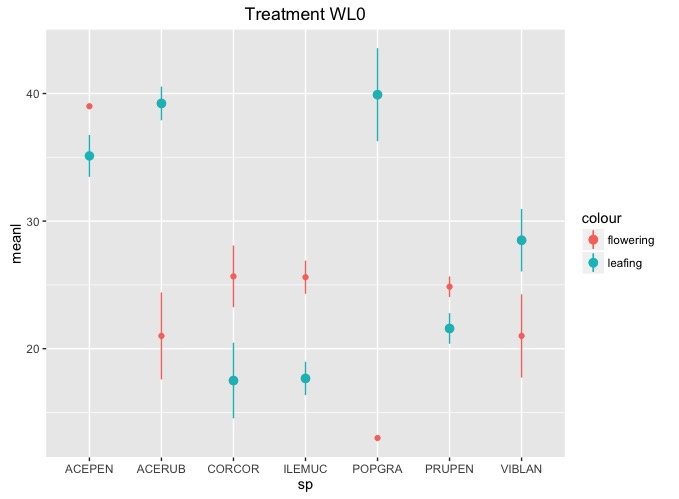
\includegraphics[width=4.5cm,height=4cm] {WL0}
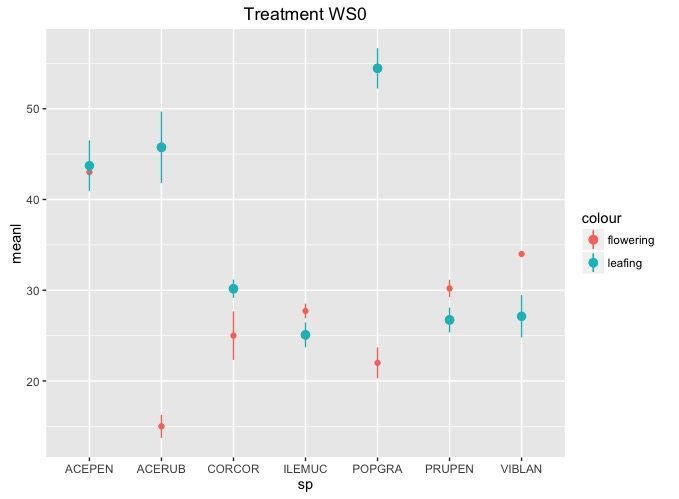
\includegraphics[width=4.5cm,height=4cm]{WS0}
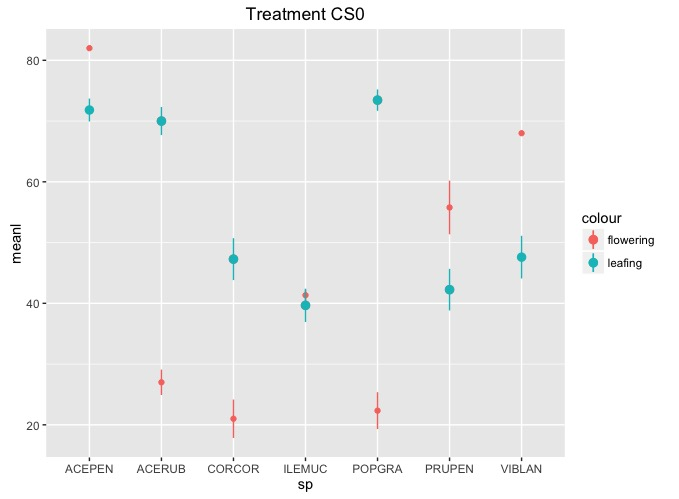
\includegraphics[width=4.5cm,height=4cm]{CS0}
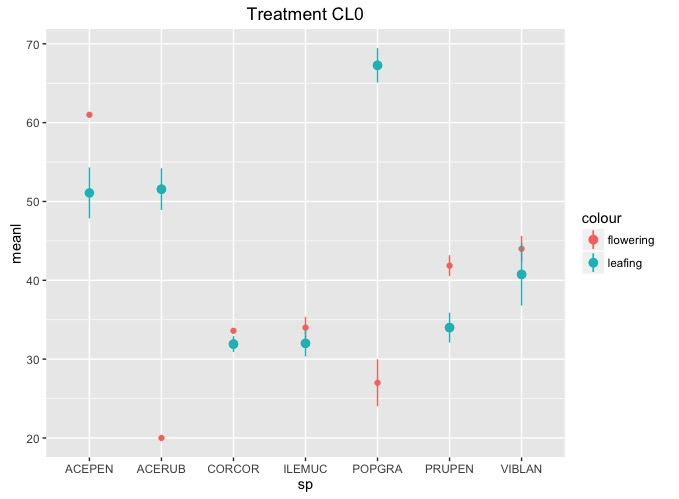
\includegraphics[width=4.5cm,height=4cm]{CL0}

These results suggest that floral and foliate phenophases can respond to the environment relatively independently of each other, each one tracking its own climate optimum. 
\par At this point in our discussion, I would like to challenge the assumption we have been holding that phenophase independence is the optimum strategy for environmental matching. In the previous section discussing maternal effects, I established the idea that a degree of offspring dependence on the conditions experience of maternal environment may allow the offspring to better "interpret" proximate environmental cues. Could this also be true between earlier and later phenophases? Could earlier phenophases serve as "sentinels", testifying to the reliability of environmental cues? For example, imagine a simplified phenological system in which in a given tree, flowers typically emerged after 200 degree days of warm temperatures and leaves typically emerged after 225. If the flowers emerged in some years and experienced a frost event, indicating the unreliability of the temperature cues for that year,  would it not be adaptive for this experience to signal or constrain leaf out, increasing its growing degree requirement and pushing it later in the season to when temperature cues would likely be more reliable? To my knowledge, there is not yet any published work exploring the possibility of sentinel effects for phenology, but preliminary data (Chamberlain, personal communication) suggests that a frost event experiences by earlier leafing buds on a given tree appears to delay bud burst in other part of the tree when compared to unfrosted trees growing in the same overall climate conditions. These sentinel buds may serve to reduce to overall risk of frost damage, but more research is needed in this area to assess the strength and effectiveness of sentinel effects in tree phenology.
\par I have now given evidence that maternal, epigenetic effects in forest trees can influence the phenology of offspring, and that climate effects of earlier phenological phases show potential to influence the timing of later phenological stages. We have discussed why both of these constraints on the plasticity of phenological expression may be adaptive to trees by providing a background "context" in which they interpret the environmental cues that govern phenology. But in an era of rapid climate change, the maternal environment may be a poor proxy for offspring environment in long lived organisms like trees, and as such, rather than conditioning offspring to respond appropriately to proximate cues, maternal effect might restrict appropriate responses to novel conditions. For example, under historic conditions, the tendency for cold maternal environments to increase the forcing requirements for spring phenology in offspring would minimize the likelihood that a winter warm spells, which would not be a reliable cue for seasonal growing optima, would cause mistimed phenological expression. However, if there was significant overall climate warming within the life time of the offspring, what were previously winter warm spells may actually be more reliable cues of optimum conditions, and the epigenetically wired delay of phenology in offspring would be a competitive disadvantage. Are phenological responses to the environment hardwired throughout a tree's lifetime, or are further epigenetic changes possible throughout a tree's development, allowing it to fine-tune its phenological response based on the accumulated experience of environmental conditions over the seasons?  
\section{Carryover effects between years}
\par As with carryover effects between phenophases, I found few studies in the literature exploring the possibility of epigenetic change of phenological patterns within the lifetime of a single organism.
Some of the studies investigating maternal effects on phenology also evaluated whether environmental conditions during the first year of seedling growth resulted in epigenetic phenotypic change related to phenology \citep{Gomery2015} and found evidence for epigenetic control of phenology based on conditions during seedling development. However, because the authors only observed the seedling stage of their experimental subjects,from these results, one cannot differentiate between the signature of a developmental carryover effect a seasonal carryover. Some evidence for a seasonal carryover effect in phenology was found by Sogaaard et al \citeyear{Sogaard2008} who showed that  bud burst timing in \textit{Picea abies} was strongly influenced by environmental conditions during the previous summer's bud set. In contrast, a study by Chuine and Cour \citeyear{Chuine1999} found that adding variables related to conditions in past years did little to improve the accuracy of predictive phenological models.
\par A more thorough exploration of carryover effects between years would be important to better predict how trees may respond to the the non-stationarity of climate change with in their own lifetimes. To further this aim, I will now present a brief research proposal for a project designed to measure phenological carryover effects across years as a response to spring frost events. This proposal differs from existing treatments of memory effects on phenology in two ways:
1) As mentioned above, most research treating memory effects in plants deals with inter-generational epigenetics. In my proposal I am seeking to identift signatures of epigenetic changes \textit{within} the lifetime of my study organisms.
2) Most memory effect studies look at the influence of past broad climate conditions on future phenotyes. By choosing to investigate the carryover effect of spring frost events, my study aims to evaluate if discrete, episodic temperature extremes can trigger similar epigenetic effects to those induced by more sustained climate conditions. The sections below will provide further background about the nature of late spring freezing events and provide an outline for the experimental methods that will be utilized to detect carryover effects from year to year.
\subsection|{False Spring Events}
The variable climate of the early spring may produce weather patterns where unseasonably high temperatures are followed by a significant temperature drop to below freezing, resulting in a false spring event when for trees, rapid vegetative growth prior to the freeze is disrupted, resulting in a post freeze phyisological setback \citp{Gu2008}.Generally, freezing events that occur during vegetative growth phenophases (between bud burst and leaf out) impose the greatest freezing threat to deciduous tree species \citep{Baslerish}. Trees that have been exposed to a false spring are likely to experience leaf loss and slower canopy development \citep{Hufkens2012}. Thus, increases in frequency or intensity of false spring conditions would increase the likelihood that a tree suffers damage from a false spring event. But might exposure to a false spring event catalyze epigenetic changes in an individual to alter their phenological pattern and reduce the chances of re-exposure in subsequent years? There are several phenotypic changes that one might expect to see if indeed such epigenetic changes had occurred. 1) Bud bust of individuals who have experienced a false spring event in the past will be delayed when compared to sympatric individuals with no frost history. 2) Individuals who have experienced a false spring event will accelerate development between bud burst and leaf out resulting in a reduced  duration of vegetative risk (DVR) when compared with unexposed sympatrics. 3) Previously exposed plants will show elevated frost tolerance during their DVR compared with trees with no history of exposure. Identifying if such changes are possible, and understanding the strength and longevity of these effects will greatly improve our understanding of the impact of frost damage over the lifetimes of a trees, which would be important across a wide variety of fields including, ecosystem modeling, forestry and conservation science.
\par I will test for phenological carryover effects between years using three species of deciduous temperate forest trees. For each species, 100 stem cutting will be obtained from natural populations, rooted in a standardized growth medium and grown under greenhouse conditions. In the spring of year 1, 50 individuals from each species will be randomly assigned to a freezing treatment, and exposed to 24 hours of freezing temperatures, while 50 other will remain unfrozen as the control group. In year 2, each group will be subdivided again with 25 from each original group receiving freezing treatment and 25 from each group not receiving the treatment. This subdivision and freezing will occur again in the year year 3, resulting in 8 groups, each with with a unique false spring history. (see figure below).\\\\
\begin{center}
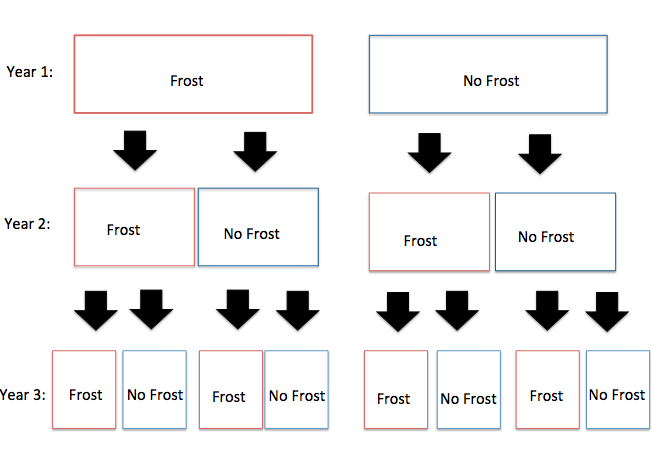
\includegraphics[width=9cm] {carryover_diagram}
\caption{Figure 2}
\end{center}
Throughout the experiment, the date of bud burst, duration of vegetative risk, and proxies for frost tolerance (anti-freeze proteins and specific leaf area after development) will be measured. Any significant differences in these response variables between treatment group would be indicative a measurable carryover effect. One shortcoming of this approach is that it does not investigate the underlying genetic architecture of carryover, so even if phenotypic changes are observed as a response to the treatments, the mechanisms producing them cannot be conclusively identified. Still, such results would be informative for the initial question of how trees may cope with increased risk from frost damage, and would suggest that further study of the mechanisms is warranted.
\section*{Conclusion}
\par Phenology allows for organisms to match important life stage transitions with optimum environmental conditions. The is evidence that epigenetic maternal effects and conditions during earlier phenological stages may constrain the phenological plasticity, but these effects vary among species and phenophases, and further research is needed to better understand the effects of and mechanisms for these constraints. In some cases, memory effects may constrain phenology of a tree to its overall fitness benefit while in other cases, such constraints may be detrimental, and these fitness effects are largely determined by the variability of the climate space in which a woody plant is growing. Additionally,the evidence for biological carryover effects between seasons or years within the lifetime of an organism is sparse and divided, and further research is needed in this area as well. Overall, it is likely that memory effects play an important role in dictating phenological responses to environmental conditions, and understanding the mechanisms and expression of biological memory and carryover effects will help us to better understand and predict the fate of forest trees in an era of global change. 


\bibliography{..//refs/278.bib}
\end{document}
